\section{Version control of artistic assets} \label{case-study-2}
At this point, the game is already working with the most important features implemented. Following the 
\href{https://docs.godotengine.org/en/stable/getting_started/first_2d_game/06.heads_up_display.html}{\color{blue}guide},
there are two additional features contributing to the experience, namely the heads-up display and sound effects, however,
the purpose of this paper is to demonstrate version control application \textbf{Helix Core}\textsuperscript{\texttrademark}
which is already fulfilled. There remains only one outstanding point, the version control of animations and other artistic
assets used for the game. This scenario plays important role when the game development includes also production of own
assets and artistic teams are also working on animations and 3D models. \hfill \break
For demonstration purposes, the sprites used for the game will be amended and see what version control techniques are 
available in \textbf{Helix Core}\textsuperscript{\texttrademark} to keep track of change.
\begin{itemize}
    \item create new stream for artistic team {$=>$} call this \textit{art1.0}
    \item observe how the development branches (streams) interact with the main branch, e.g. changes in artistic elements
    copied to main and from there, merged to the other development stream used by game programmers.
\end{itemize}
\begin{figure}[H]
    \centering
    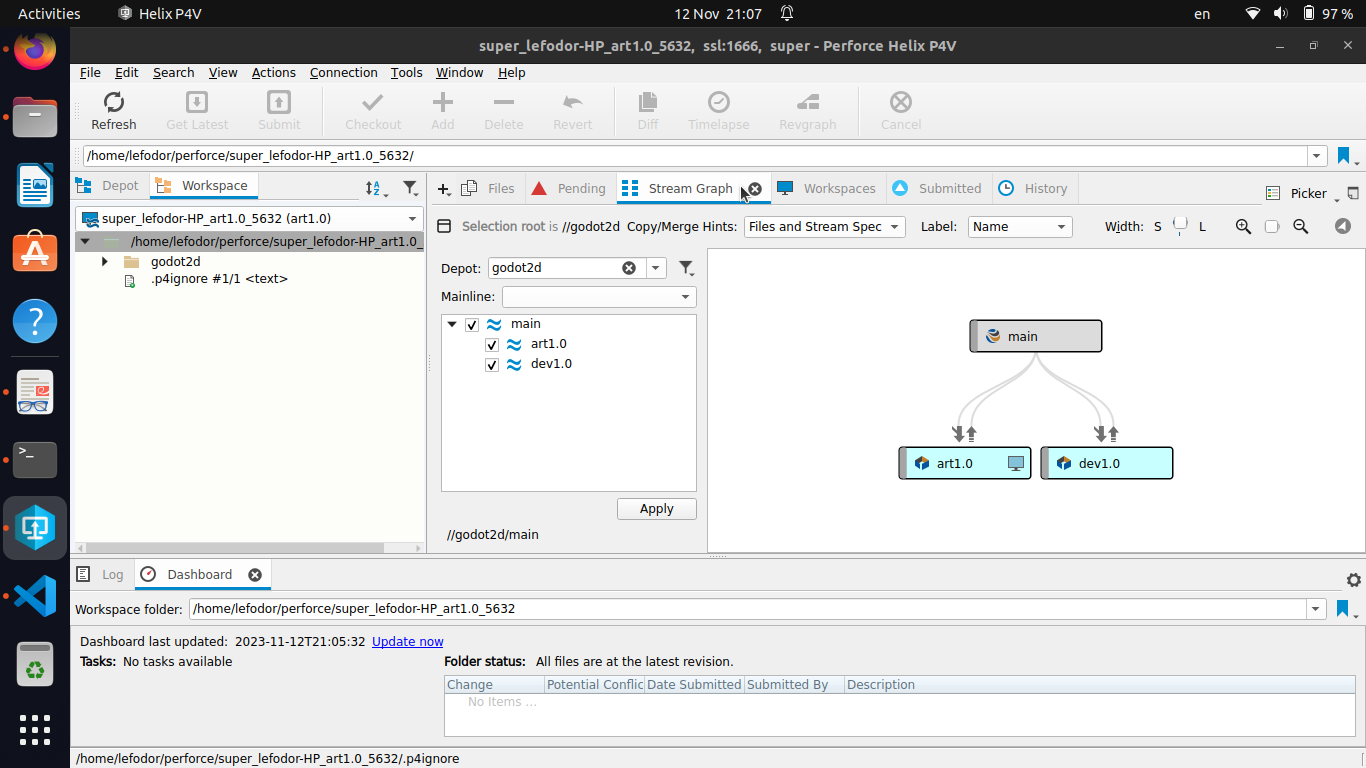
\includegraphics[width=\textwidth]{new-art-stream-created.png}
    \setlength{\belowcaptionskip}{-10pt}
    \caption{new art stream created}
    \label{fig:new-art-stream-created}
\end{figure}
At the moment, all up- and downstream arrows between the streams are gray, indicating there are no differences that need
synchronization. Let's check out the \textit{art} directory in from the \textit{art1.0} workspace and try to make some
changes to the player's sprite \hfill \break (\$workspace/godot2d/art/playerGrey\_*.png). %\hfill \break
\begin{figure}[H]
    \centering
    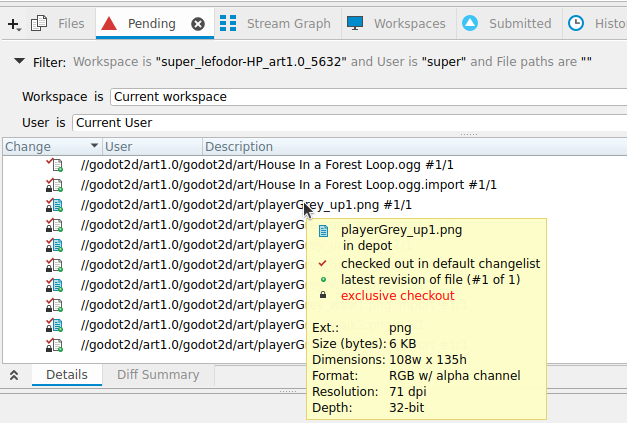
\includegraphics[scale=0.5]{assets-checked-out.png}
    \setlength{\belowcaptionskip}{-10pt}
    \caption{assets checked out}
    \label{fig:assets-checked-out}
\end{figure}
The .png files are all checked out with exclusive flag, meaning that they cannot be checked out simultaneously 
in multiple workspaces hence no parallel editing is possible. This property is defined in the Typemap file in
\ref{setup-version-control}. Submit the modified files and update the streams:
\begin{figure}[H]
    \centering
    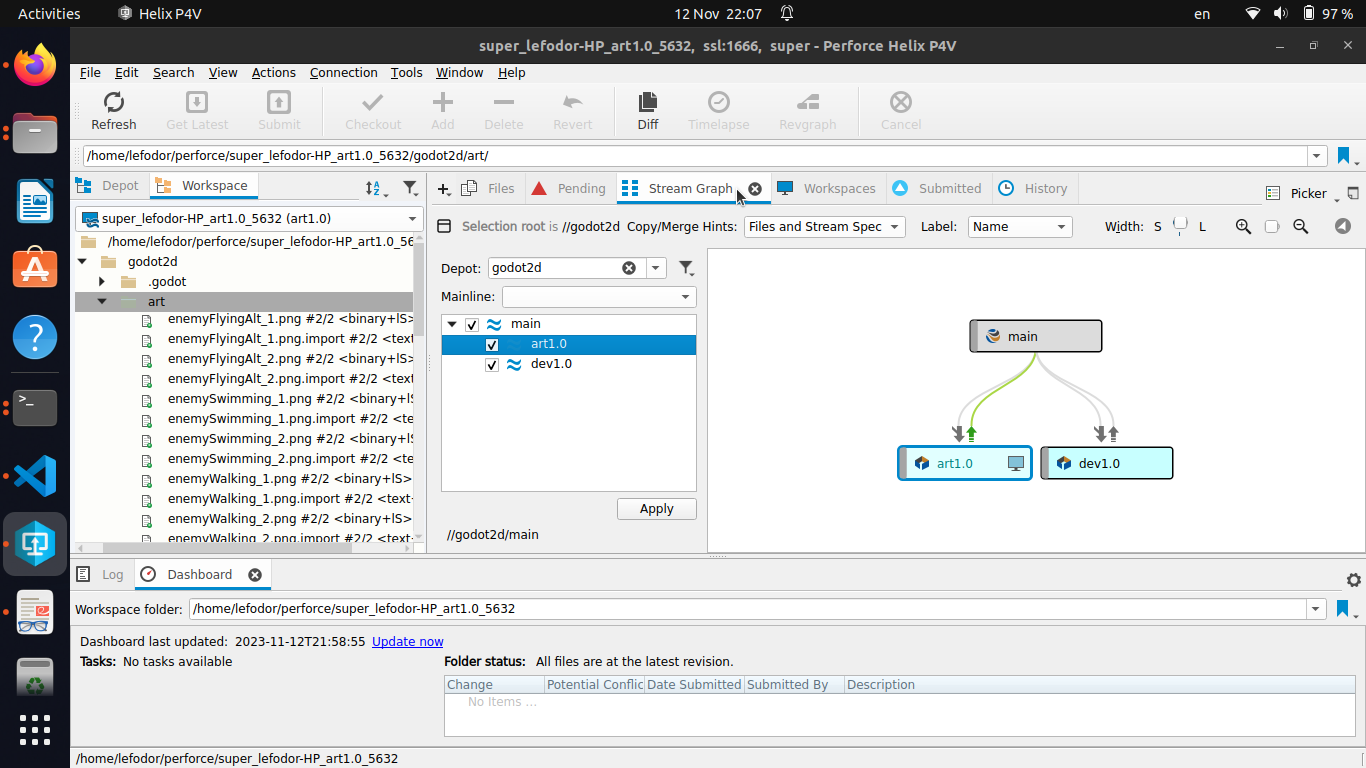
\includegraphics[width=\textwidth]{assets-modified-streams.png}
    \setlength{\belowcaptionskip}{-10pt}
    \caption{assets modified streams}
    \label{fig:assets-modified-streams}
\end{figure}
This time, the green arrow shows up between streams \textit{main} and \textit{art1.0}, indicating that the latter has
changed and the modified files can be copied to main. Copy the modified files from \textit{art1.0} to \textit{main}, 
and submit the changes so that they take effect.
\begin{figure}[H]
    \centering
    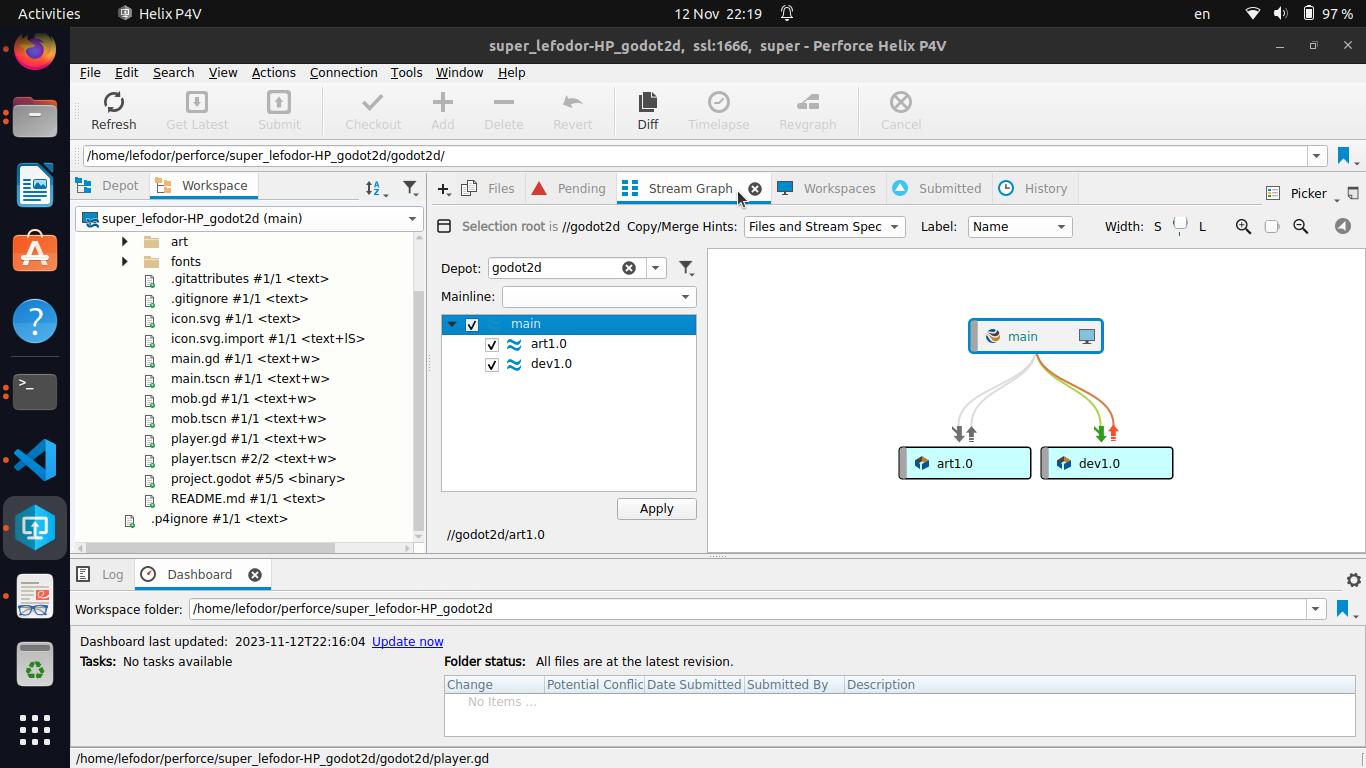
\includegraphics[width=\textwidth]{assets-change-main-dev.png}
    \setlength{\belowcaptionskip}{-10pt}
    \caption{assets change main dev}
    \label{fig:assets-change-main-dev}
\end{figure}
As can be seen, the changes of from \textit{art1.0} propagate to all other streams via \textit{main} and require 
synchronization so that it go to all working streams in the project. This can be done by following the steps set out in
the previous sections.